\documentclass[aps,letterpaper,11pt]{revtex4}

\usepackage{graphicx}
\usepackage{float}
\usepackage{verbatim}
\usepackage{amsmath}
\usepackage{amssymb}

\newcommand{\labno}{1}
\newcommand{\labtitle}{Analyzing Graphical Representations of One Dimensional Kinematics Using Logger Pro}
\newcommand{\authorname}{Kevin Truong}
\newcommand{\professor}{Dr. Melanie Lutz}
\newcommand{\classno}{Physics 006}
\newcommand{\labpartners}{Adam Walker, Ben Mendiola, Kwihyeong Kang}
\newcommand{\submitdate}{January 31,2017}

\begin{document}

\begin{titlepage}
\begin{center}
\hspace{-136mm}\boxed{{\Large \textsc{Lab No. \labno}}}\\\vspace{30mm}
{\Large \textsc{\labtitle} \\ \vspace{4pt}}
\rule[13pt]{\textwidth}{1pt}\\ \vspace{150pt}
{\large By: \authorname \\ \vspace{10pt}}
Lab Partners: \labpartners \\
Instructor: \professor \vspace{10pt} \\
Solano Community College\\ \classno \\ \vspace{10pt}
\submitdate
\end{center}
\end{titlepage}

\section{Abstract}

Graphical representations of one dimensional motion can be analyzed by using the Logger Pro program and a sensor. With the use of the program, it was possible to quantify movements towards and away from the sensor. Understanding that moving away from the sensor prompted positive outputs while movement towards the sensor prompted a negative output. From these graphs, it was possible to derive the velocity and acceleration. The velocity of the graphs was obtained by looking at the slope of the position vs. time graph while acceleration was obtained by observing the curvature. Initially we observed position vs time graphs that had variable velocity and acceleration, this was achieved by using a flat surface and walking in front of the sensor to simulate one dimensional kinematics. It was observed that walking quicker and slower in front of the sensor caused the slope of the position vs. time graph to change depending on the speed of the movement. The experiment was concluded with the observation of a system with an acceleration of 0 $\frac{m}{s^2}$, this was achieved by using a cart on a flat "frictionless" ramp creating constant velocity. With the cart and ramp, we observed a linear position vs. time graph indicating a constant velocity because its uniform slope throughout.

\section{Introduction}
One dimensional kinematics may be seen as simple; however, it's the concepts in one dimensional systems that build the basis of 2nd, 3rd, and nth dimensional kinematics. Movement, no matter the dimension, will have position, velocity, and acceleration relative to an origin. The complexity of studying kinematics can be amplified by looking at inconsistent acceleration. Unfortunately, the majority of movement, in the real world, is modeled with varying acceleration. Without knowing a function that represents this acceleration, it's a necessity to be able to understand the graphs that model the movement. 

When looking at variable acceleration, it is understood that velocity and position will also be variable. Since velocity is not uniform throughout, velocity can be examined as average velocity or instantaneous velocity. Average velocity is data over a certain interval of time while instantaneous velocity is data at a single point. Average velocity is understood to be the change in displacement($\Delta x$) over the change in time($\Delta t $), modeled by $\bar{v} = \frac{\Delta x}{\Delta t}$. While instantaneous velocity can be acquired by looking at the tangent line at a specific point.

\newpage

\section{Experimental Details}

Equipment for this experiment includes a computer, Logger Pro Program and hardware, sensor, textbook, meter sticks, cart, and flat ramp. The computer was used to run the Logger Pro program and display the data collected. The Logger Pro Program and hardware were used to collect and organize data from the sensor. The sensor was used to read motion, and was the origin. The textbook was used as a flat surface, so the sensor would have an easier time detecting the motion created by us. The meter stick was used to measure the distance away from the sensor since some scenarios in the experiment prompted us to begin a certain distance away from the sensor. The cart and ramp were used to model a system with constant velocity, the "frictionless" ramp was a medium that allowed the cart to achieve constant velocity.



\subsection{The Diagram of motion detected by sensor}

\begin{center}
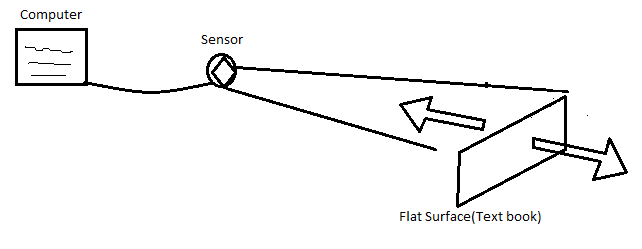
\includegraphics[width=4in]{DIAUS.png}
\end{center}

It's important to note that the sensor uses ultrasonic waves in a cone of 15-20$^\circ$ and will detect the closest object. It's also important to note that since the sensor is only detecting what's in front of it, we're only looking at positive positional values. Therefore the words distance and position will both be used in this experiment and are interchangeable in this context.  


\section{Procedures, Results and Analysis}

\subsection{Distance vs. Time Graphs}

In section A, the graphs displayed on the Logger Pro program were strictly limited to Distance vs. Time. Initially, the behavior of these graphs was understood by practicing linear movements in front of the sensor. We compared the effects of walking slowly vs. quickly and walking away vs. walking towards in front of the sensor. The faster the motion the steeper the slope, quicker change in position in respect to time. The direction of the slope depended on if the motion was walking away or towards the sensor. Since the sensor is the origin, walking away from the sensor created positive slopes while walking towards the sensor created negative slopes. 

After understanding the basics of motion in front of the sensor, we were challenged to predict the line for a given scenario. The scenario being a starting position of 1.0m in front of the sensor then moving at a constant velocity away from the sensor, then stopping, and finally moving at a quicker constant velocity towards the sensor. Figure 1 is the distance vs. time graph that models this scenario.


\begin{center}
Figure 1\\
\vspace{-20mm}
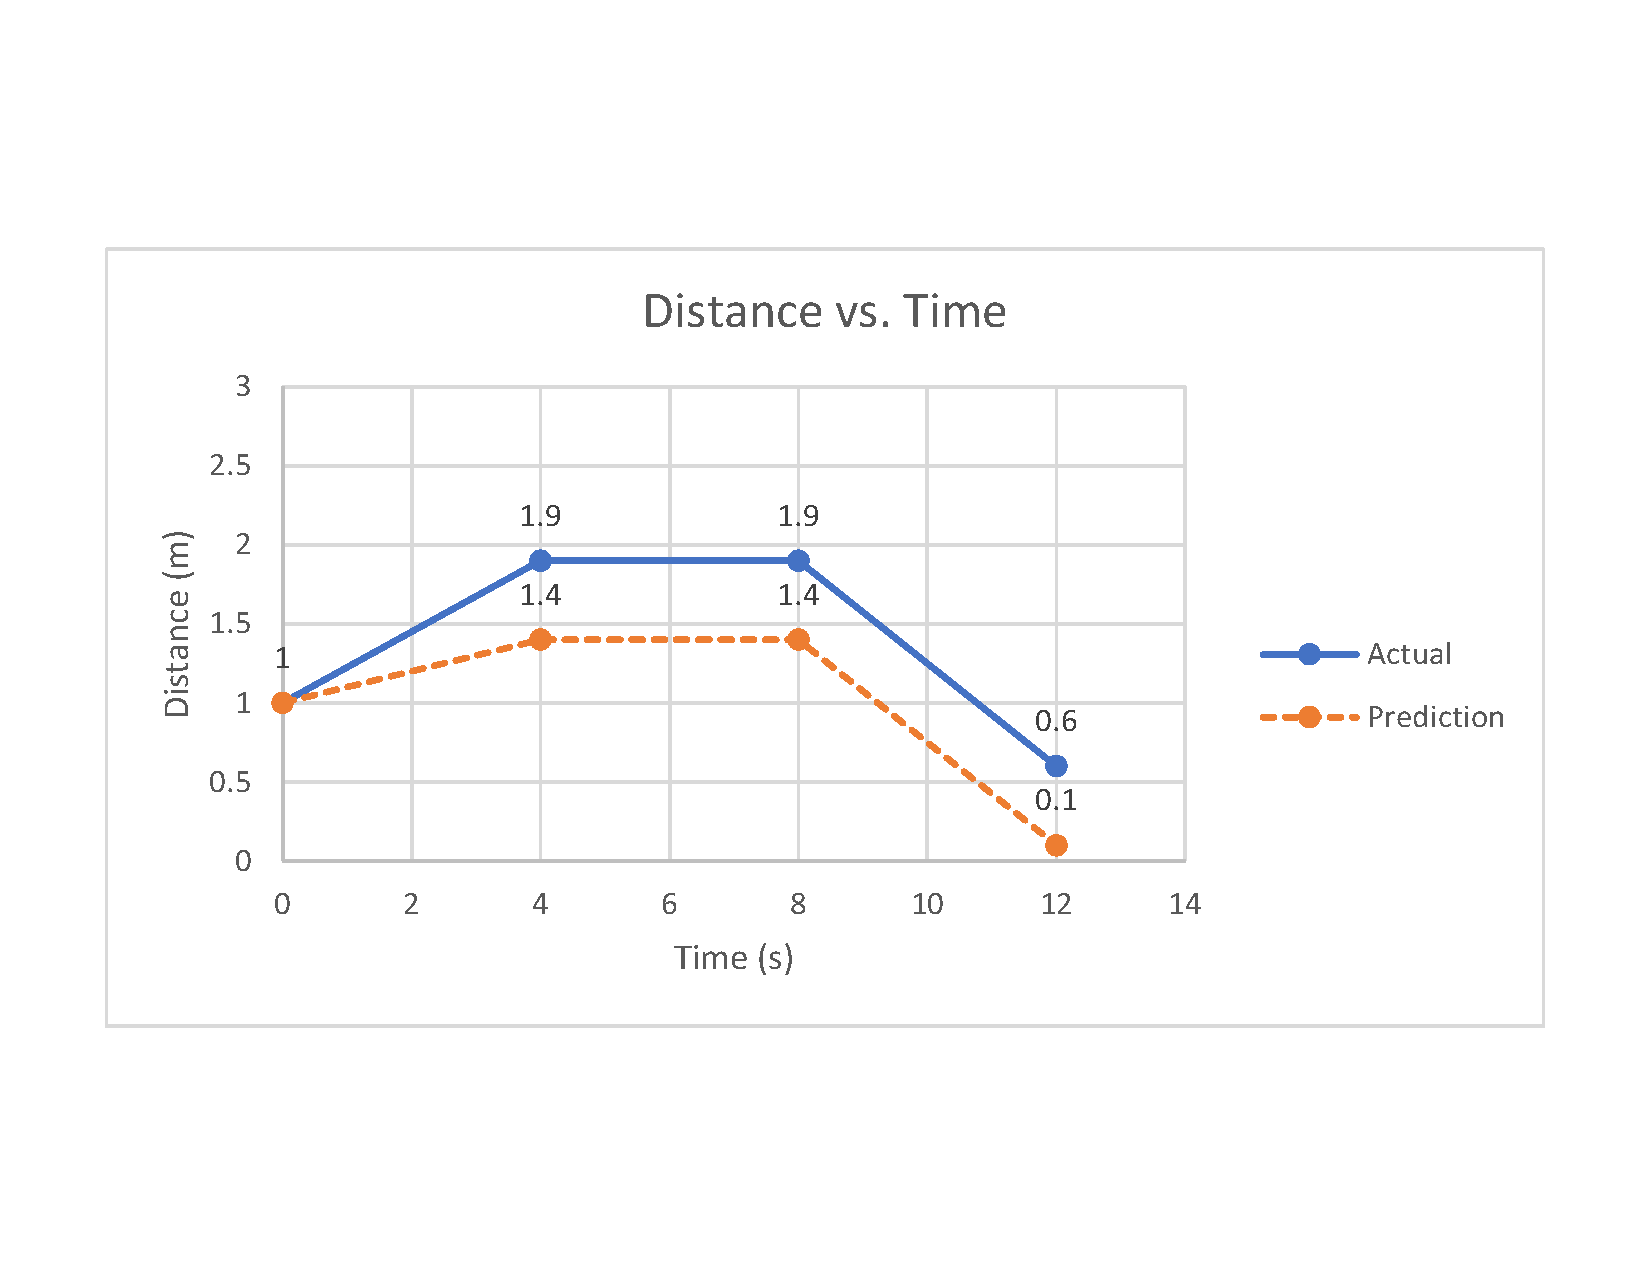
\includegraphics[width=6in]{Graph1.pdf}\\
\vspace{-20mm}
\textit{Figure 1: The distance vs. time graph for the scenario described. The dashed line was my prediction while the solid line modeled the actual output}
\end{center}

My prediction was very similar to the actual output. The difference between the two lines is the velocity of the motion, I predicted that the velocity would be slower when having a constant velocity, so my slopes were not as steep in the distance vs. time graph. The scenerio tested the production of a graph when given a particular scenario, it is also important to be able to describe the motion of a particle by looking at its graph. The process of describing a graph is just the process of creating a graph based on scenario, but working backwards. Looking at the slopes of the graph will explain the movement of the particle.

In Figure 2 presents two graphs, one graph that has constant change in position in respect to time and one graph that had increasing change in position in respect to time. The linear graph has a constant velocity, this can be explained by the uniform slope that it has throughout the interval of time. The parabolic graph has a velocity that is increasing over the interval of time, this can be explained by the  positive change in slope throughout the graph. 

\begin{center}
Figure 2\\
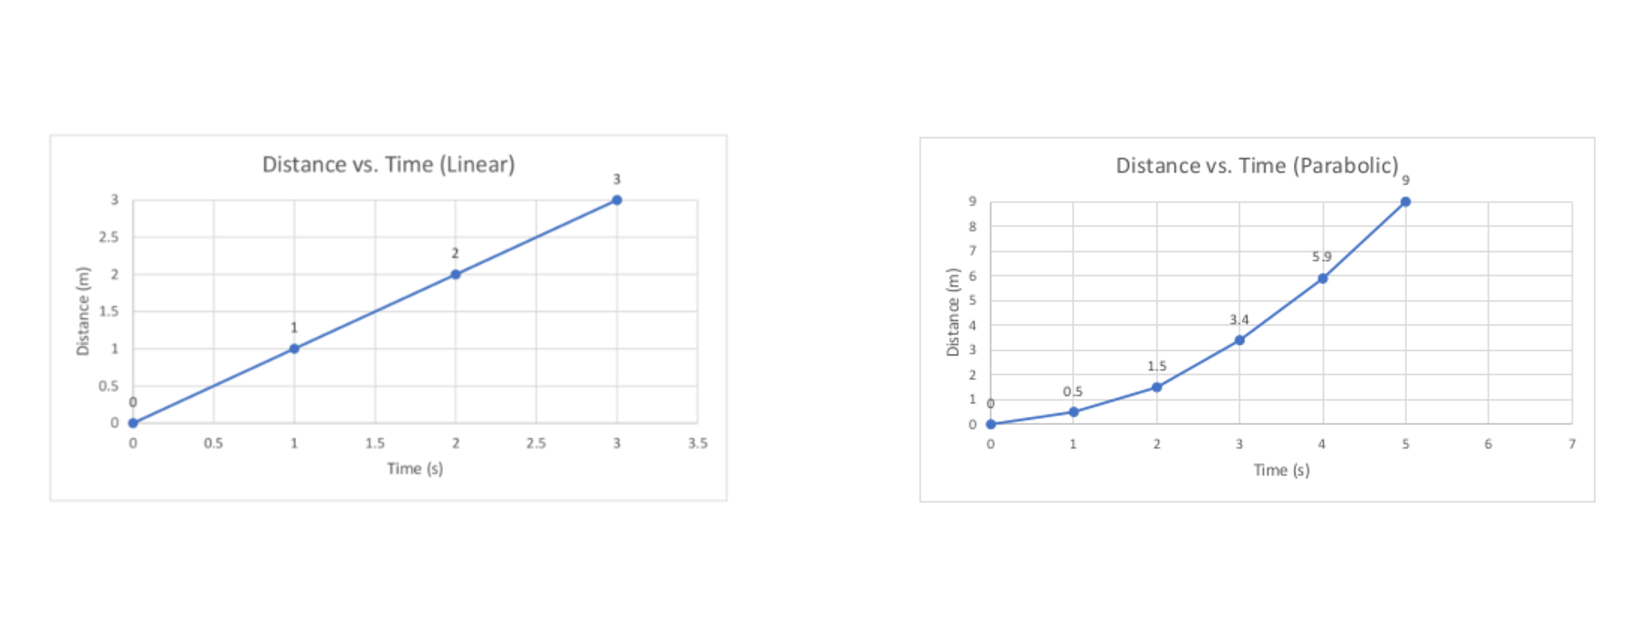
\includegraphics[width=7in]{LinearandParabolic1.pdf}\\
\textit{Figure 2: The linear graph(on the left) has a uniform slope throughout, modeling constant velocity, while the parabolic graph(on the right) has varying slopes throughout, modeling increasing velocity.}
\end{center}

\subsection{Velocity vs. Time Graphs of Your Motion}

This section focuses on velocity vs. time graphs. An important difference between a distance vs. time graph and a velocity vs. time graph is velocity does not show the distance away from the origin.  Velocity is the rate at which position changes in respect to time, so velocity(v) is the derivative of position(x) in respect to time; this statement can also be modeled by $v = \frac{dx}{dt}$. This mathematical statement explains that the velocity(v) at any point in time can be found by looking at the particular point's slope(tangent line) on the distance vs. time graph. 

Velocity is a vector quantity, so it is important to note the direction in which the movement is taking place. When looking at constant velocity, the velocity vs. time graph has a straight line through a single y-value. In respect to the origin, movement away from the sensor will prompt positive velocity values while movement towards the origin prompts negative velocity values. The y-value depends on the actual speed that describes the motion, faster movement prompts a larger value in respect to the direction of the movement. 

After understanding the basics of how movement in respect to the sensor(origin) effects the velocity graph, we were prompted to predict the velocity vs. time graph of a scenario. The scenario included walking away from the sensor slowly at a constant velocity for six seconds, then standing still for 6 seconds, and then walking towards the sensor but with twice the velocity. Since it was constant veloctiy when moving away and towards the sensor, it was easy to predict that for those intervals of time it would be a horizontal line through some y-value. It could also be predicted that the constant velocity away from the sensor would be above the x-axis and the constant velocity towards the sensor would be a value below the x-axis. There should also be an interval of six seconds between the two movements where the velocity will be horizontal at the x-axis because there is no velocity at rest. Figure 3, is a comparison of my prediction(denoted by the dashed line) and the actual result(denoted by the solid line). My prediction and the acutal result are very similar besides the value in which the horizontal line, indicating the constant velocity, was fixated upon. I predicted a slower constant velocity than actually done in the experiment. 

\begin{center}
Figure 3\\
\vspace{-10mm}
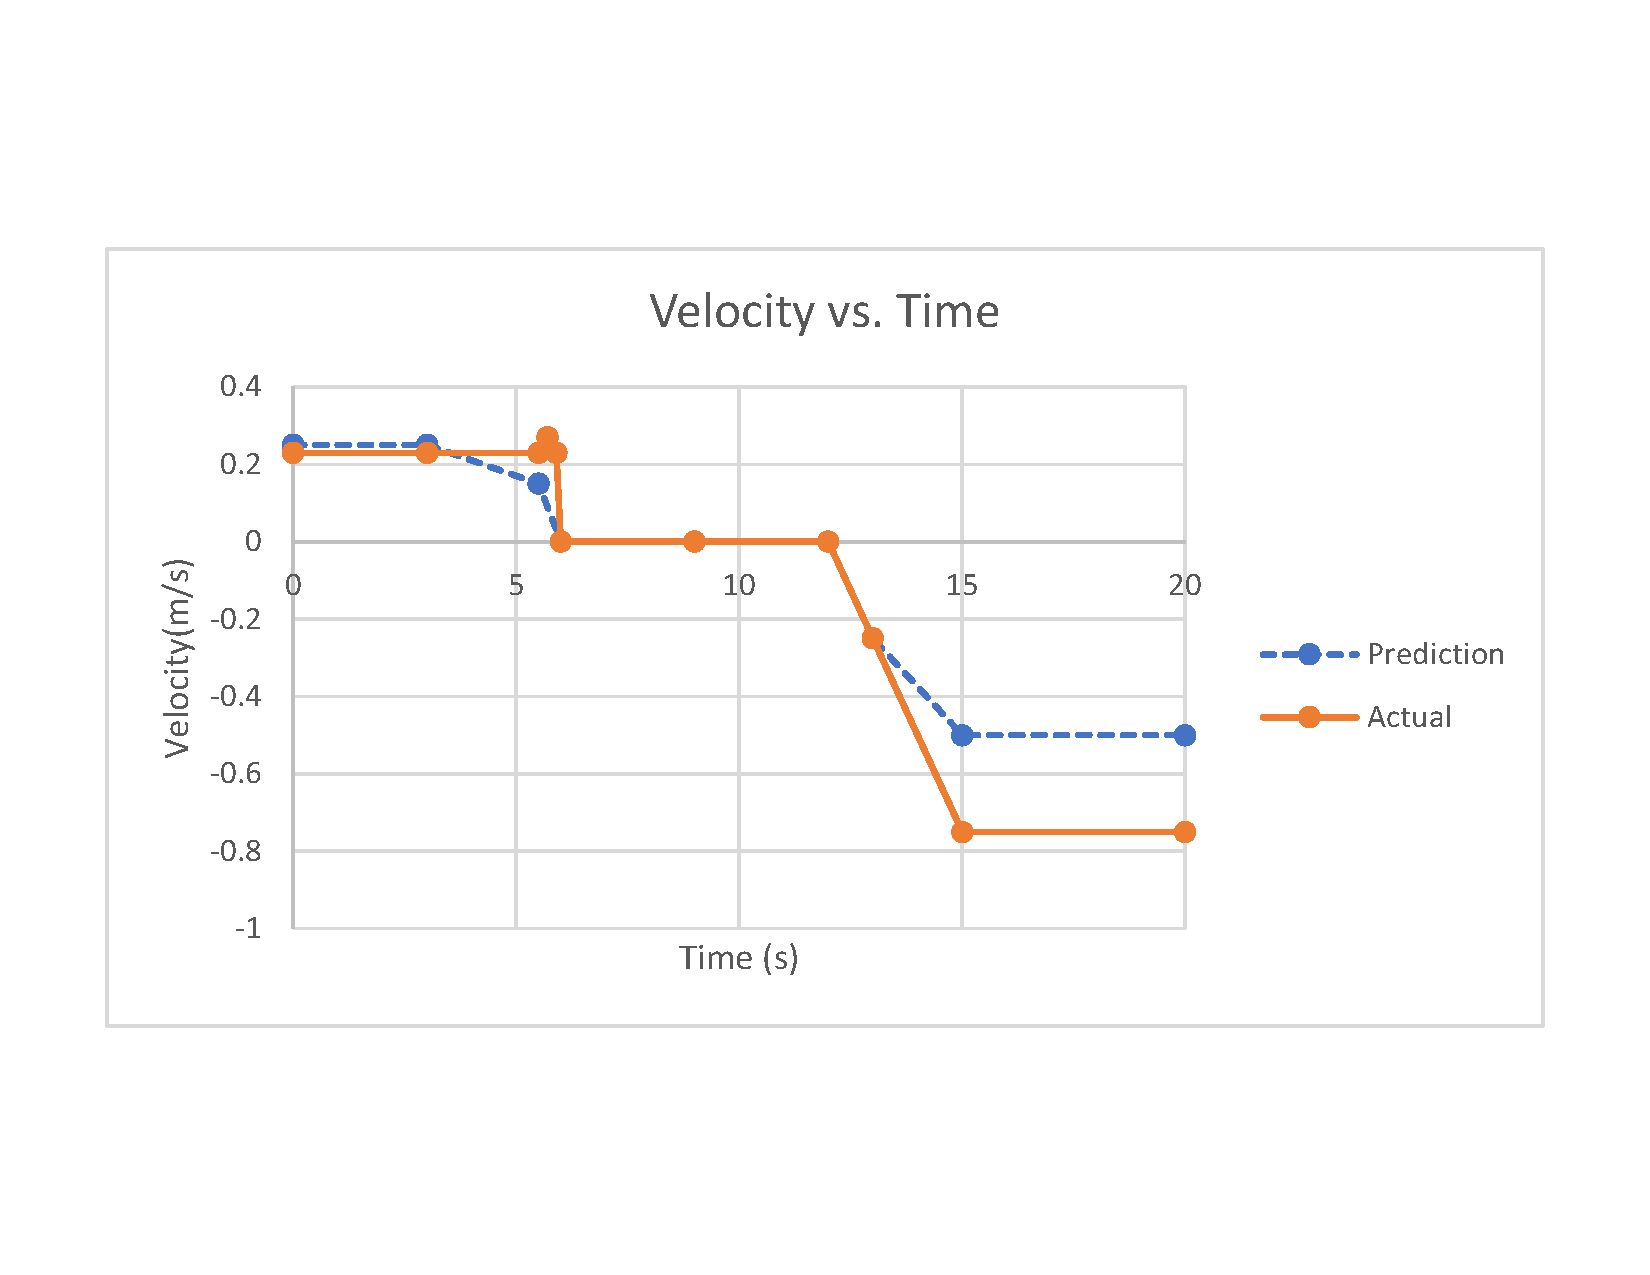
\includegraphics[width=5in]{velocityvstimeprediction.pdf}\\
\vspace{-10mm}
\textit{Figure 3: Velocity vs. time graph containing my prediction of the scenario, indicated by the dashed line, and the actual data from the experiment, indicated by the solid line.}
\end{center} 

Since velocity is a vector quantity, it can be represented by a vector. As a vector, it will have a direction and magnitude. The direction of the vector will be dependent on where the origin is placed, and the magnitude represents the value of the velocity. Figure 4 is a diagram representing velocity vectors in respect to the origin; the diagram places the origin at the left-most point of the line and the positive direction to the right, so a positive velocity vector would point towards the positive direction and a negative velocity would point towards the origin. Both of the velocity vectors have about the same magnitude, so the length of the vector is about the same.

\newpage

\begin{center}
Figure 4\\
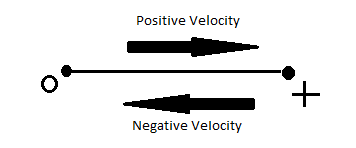
\includegraphics[width=4in]{VelocityVectorEx.png}\\
\textit{Figure 4: Diagram of positive and negative velocity vectors with respect to the origin}
\end{center}

\vspace{5mm}

Some velocity vs. time graphs are impossible to replicate in the physical world. Figure 5 would be impossible to replicate, physically, because it is impossible to instantly change velocities from \\0 $\frac{m}{s}$ to $\frac{3}{10} \frac{m}{s}$ or -$\frac{4}{10} \frac{m}{s}$. It's impossible to go from one velocity to a different velocity within no interval of time. Since the velocity vs. time graph doesn't show any positional values, it will not indicate where the system began or stopped. When attempting to replicate the graph in figure 5, we almost ran into the sensor because we thought that we had to start a certain distance away from the sensor; to combat this problem we should have started a farther distance away from the sensor.

\begin{center}
\vspace{10mm}
Figure 5\\
\vspace{-10mm}
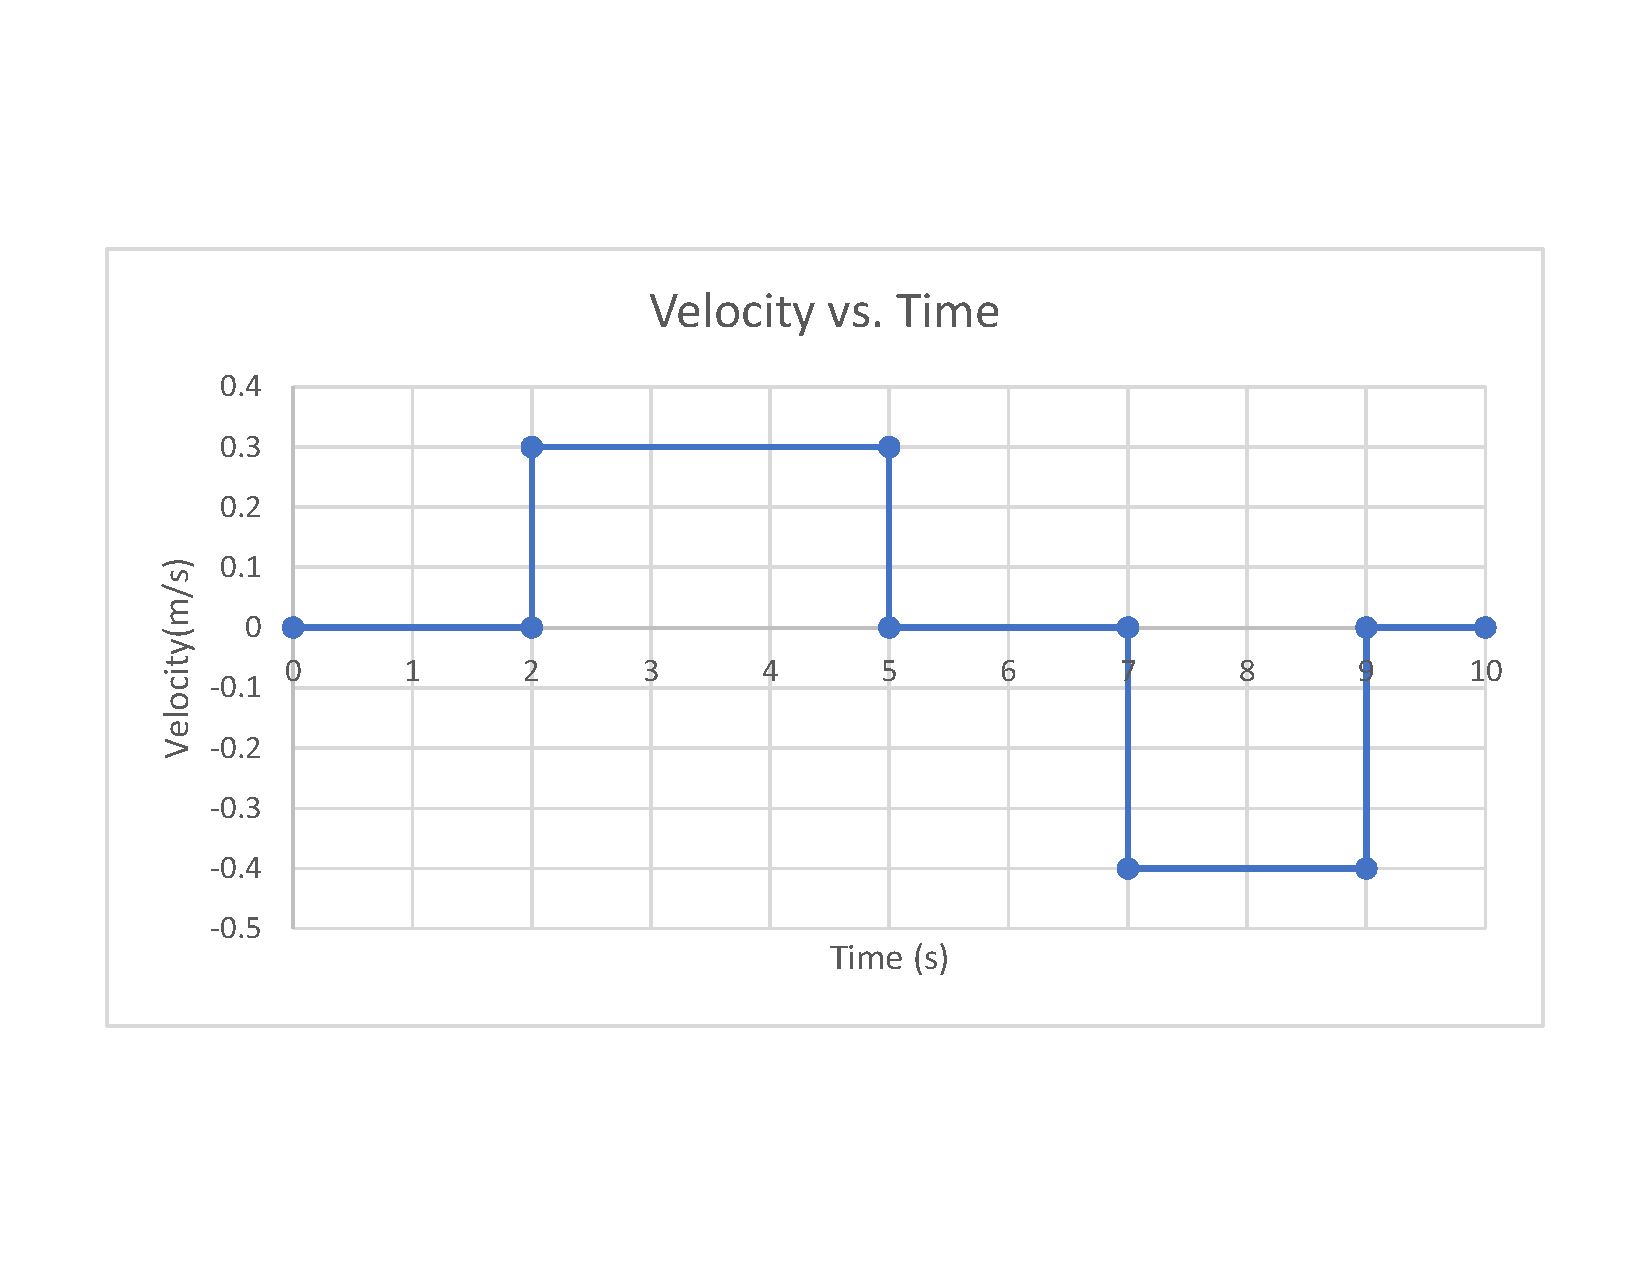
\includegraphics[width=5in]{ImpossibleVelocityVsTimeGraph.pdf}\\
\vspace{-10mm}
\textit{Figure 5: Velocity vs. time graph that is impossible to replicate in the physical world.}
\end{center}

\newpage 

\subsection{Relating Position and Velocity Graphs}

This section compares distance vs. time graphs and velocity vs. time graphs. From examining a distance vs. time graph, it is possible to predict a velocity vs. time graph. It is also possible to predict the distance away from the starting position when studying a velocity vs. time graph. When predicting a velocity vs. time graph given a distance vs. time graph, it's important to examine the slope at certain intervals of time. The slope at a particular point in the distance vs. time graph is the velocity. It's important to note that a horizontal line on the x-axis of the velocity vs. time graph represents zero positional change in respect to the origin. 

Figure 6 was a given distance vs. time graph and figure 7 was the prediction of the velocity vs. time graph of the graph represented in figure 6. In figure 7, the dashed line was the prediction while the solid line was the actual result. The prediction was slighlty different because the slope in the distance vs. time graph seemed to have a value of one, but in actuality the slope was less so the value for velocity was less. 

\begin{center}
Figure 6\\
\vspace{-10mm}
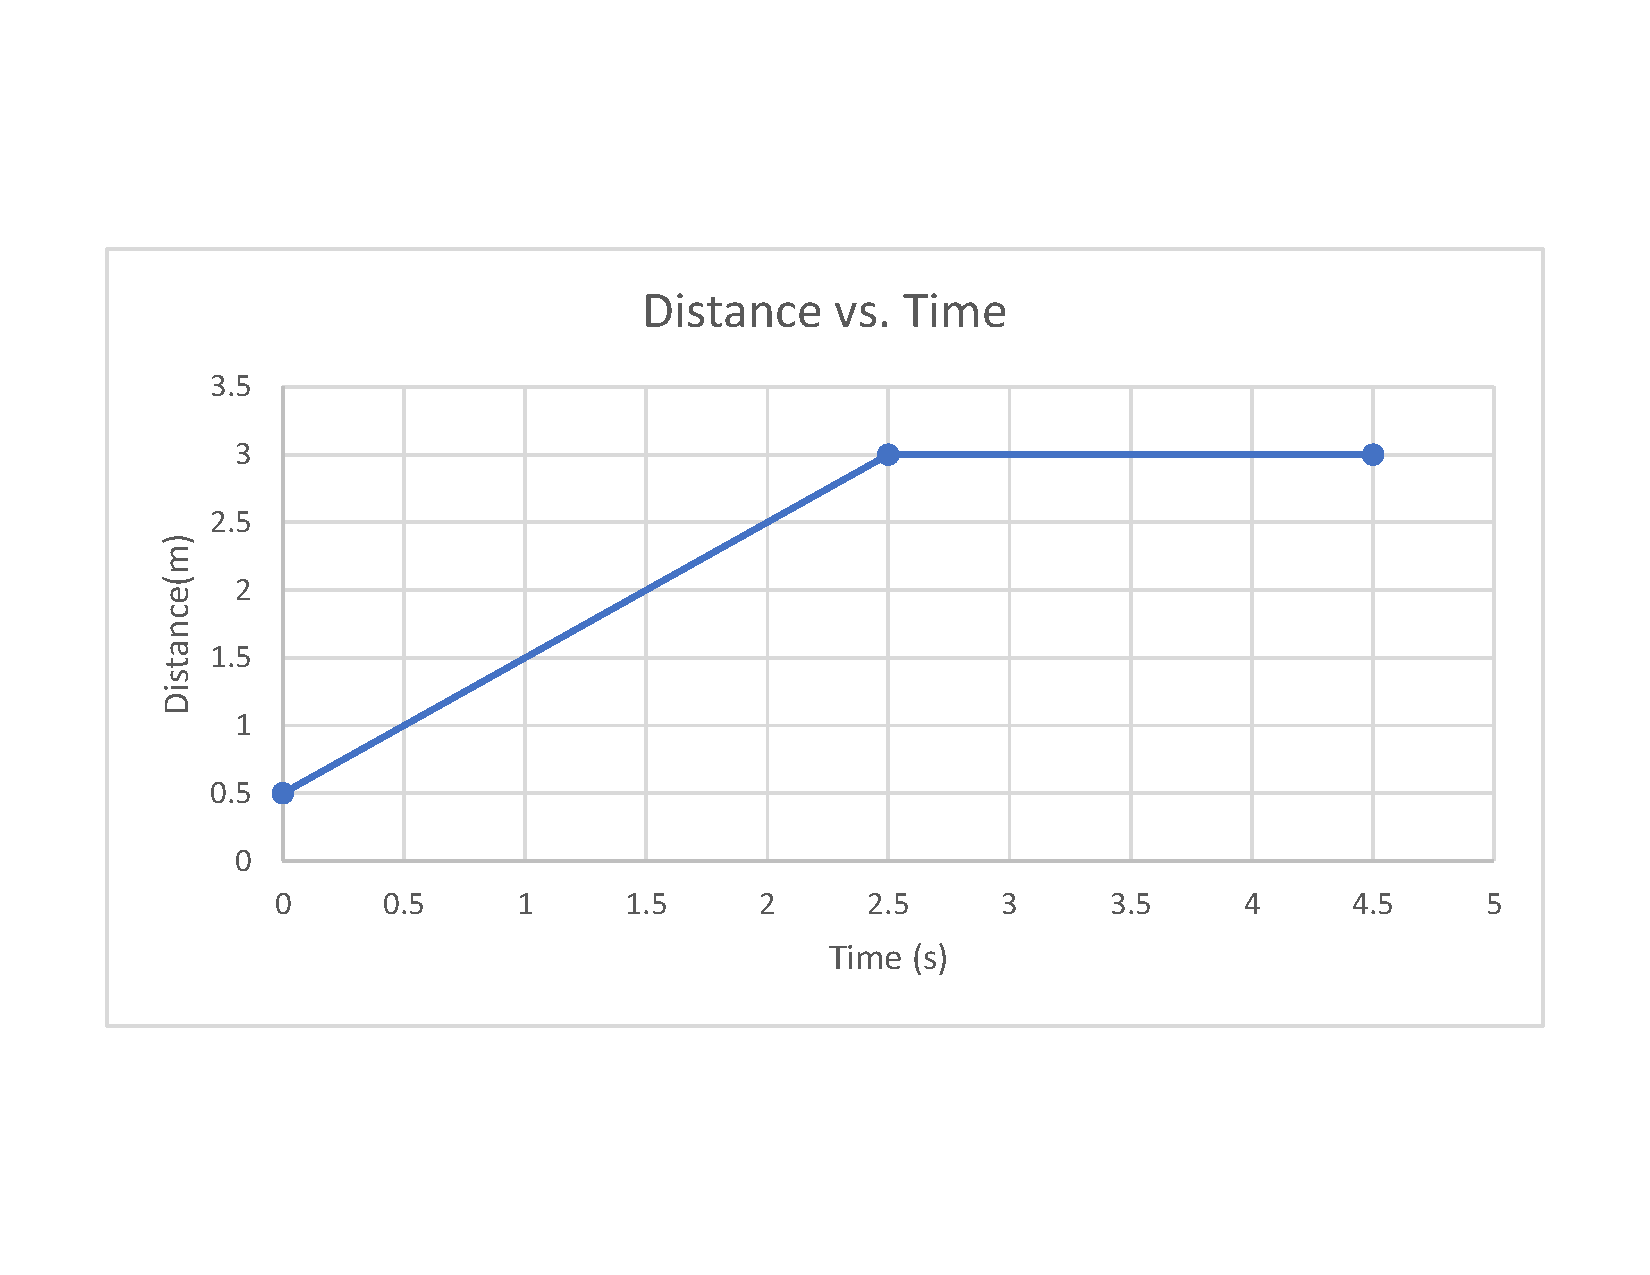
\includegraphics[width=5in]{PositionVsTimeForPartC.pdf}\\
\vspace{-10mm}
\textit{Figure 6: Given Distance vs. time graph}\\
\newpage
Figure 7\\
\vspace{-10mm}
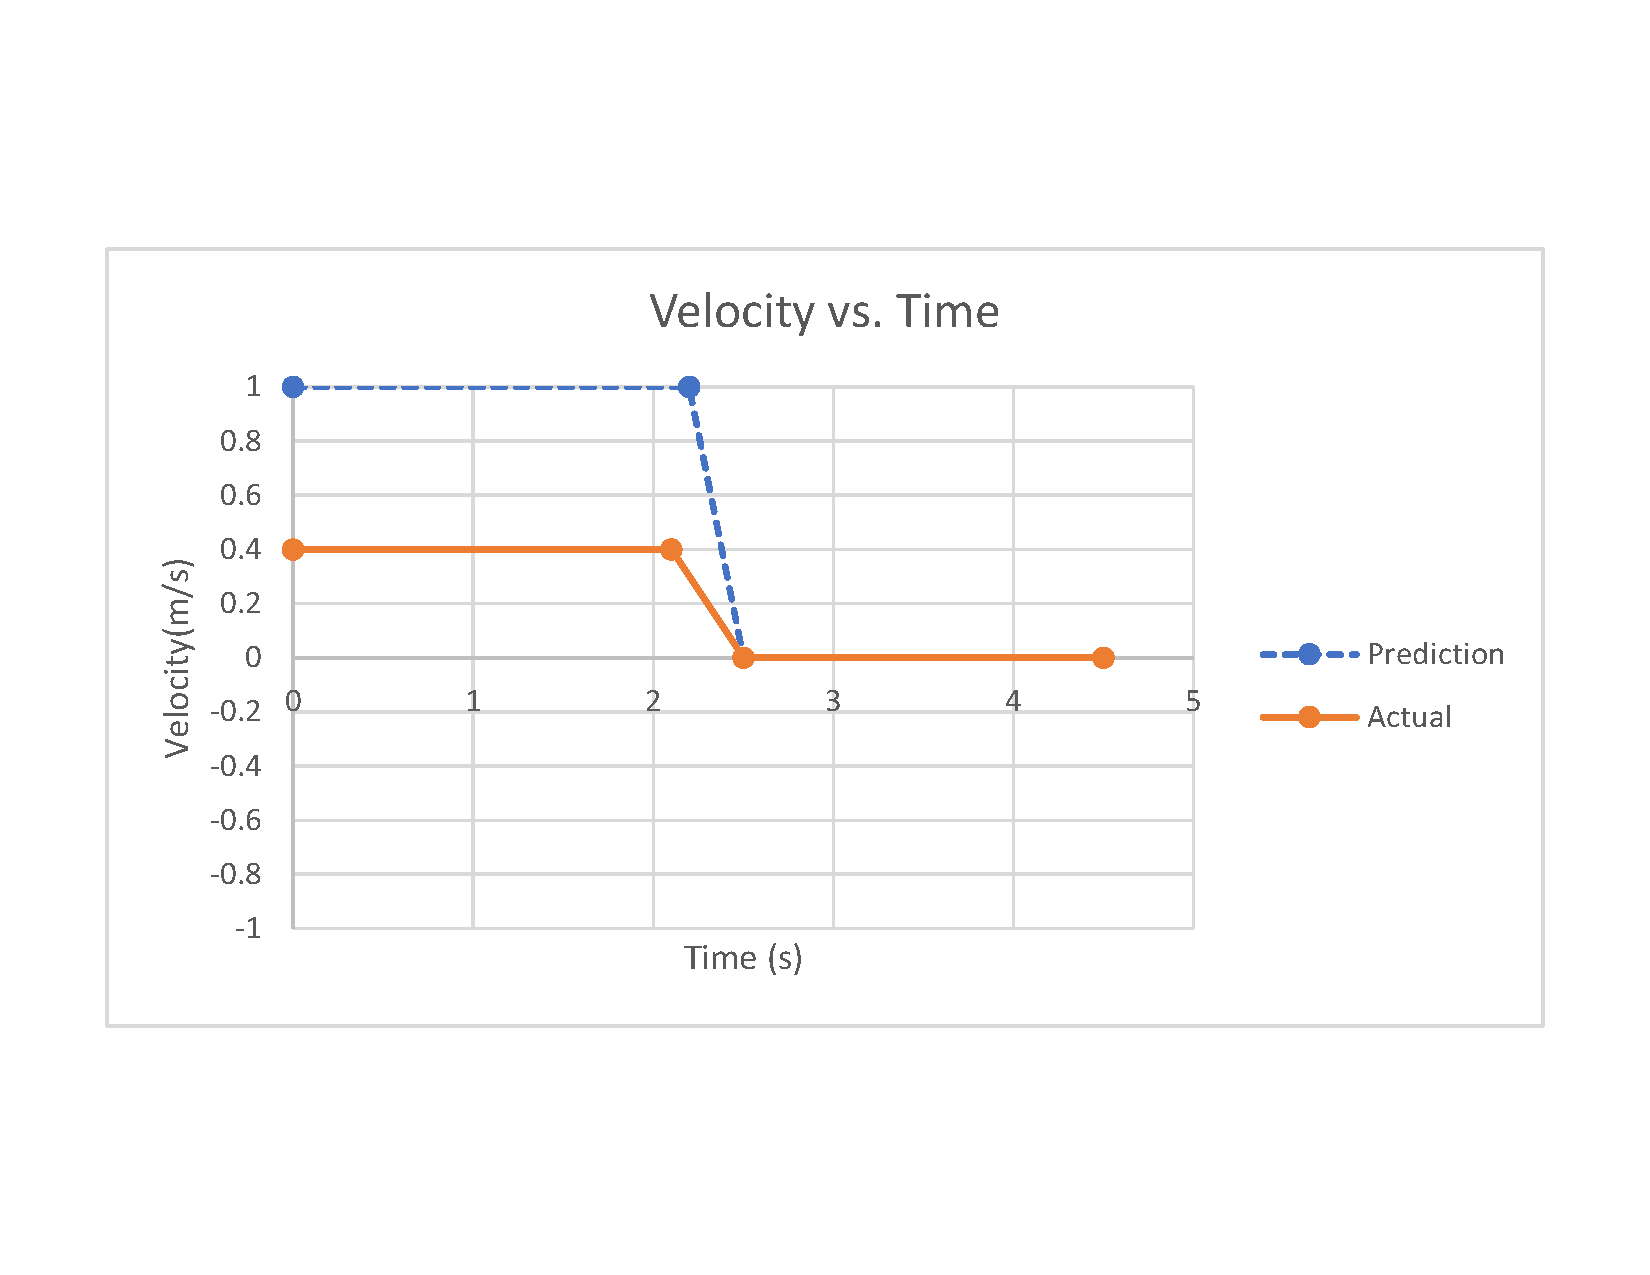
\includegraphics[width=5in]{VelocityVsTimeGraphForPartC.pdf}\\
\vspace{-10mm}
\textit{Figure 7: The velocity vs. time graph, with a line representing a prediction(dashed line) and a line representing the actual result(solid line) from running the experiment}
\end{center} 

Up to this point, the velocity being expressed throughout the experiment was instantaneous velocity. Another type of velocity is average velocity, and it is defined by a change in displacement over a change in time. Average velocity can be calculated by looking at either a distance vs. time graph or a velocity vs. time graph. When looking at a distance vs. time graph, average velocity over a certain interval is calculated by the final position minus the starting position over the change in time, the mathematical representation would be: $\bar{v} = \frac{x_1 - x_0}{\Delta t}$. Average velocity over a certain amount of time is calculated, when looking a velocity vs. time graph, by taking instantaneous velocity values across the interval and finding an average; this is done by adding up all of the values and dividing by the amount of velocity values. 

Using the methods discussed, calculating and analyzing the average velocity for graphs in figure 6 and 7 were made possible. First an estimated average velocity was calculated by looking at the velocity vs. time graph and collecting ten instantaneous velocity values and adding their values and dividing by ten, we obtained an estimated value of .356$\frac{m}{s}$. Next we used the Logger Pro program to find the average velocity over the interval of time and the program found that the average vel ocity was .355$\frac{m}{s}$, the program uses mroe than just ten instantaneous velocity values. After analyzing the velocity vs. time graph, average velocity was found by looking at the distance vs. time graph. Over the interval of time, the position vs. time graph had a right bound and a left bound indicated the distance traveled. Taking the values of both of the bounds the change in displacement was calculated, and since we knew the interval of time it is possible to calculate the average velocity. plugging into the equation $\bar{v} = \frac{x_1 - x_0}{\Delta t}$ the estimated average velocity was .348$\frac{m}{s}$ The calculation was fairly different because the bounds were accidentally altered, slightly, when analyzing the graph. The third estimate of average velocity was obtained by looking at the slope of the linear equation formed by the time interval in the distance vs. time graph. This estimated average velocity value was .354 $\frac{m}{s}$. All of the estimated average velocities were very close to eachother, this means that the methods that were used to calculate them were legitimate.

It is also important to be able to predict a distance vs. time graph when looking at a velocity vs. time graph. When looking a velocity vs. time graph with the intentions of creating the distance vs. time graph, it is important to have the intial distance away from the origin to have the starting position. A nonzero horizontal line on the velocity cs. time graph is constant velocity, so a uniform slope should be represented in the position vs. time for the interval that the velocity is constant. If there is a horizontal line at zero on the velocity vs. time graph, the object being analyzed is standing still with zero velocity. A linear slope on a velocity vs. time graph indicates that the velocity is increasing(positive slope) or descreasing(negative slope) steadily depending on the direction that it's sloping towards, a negative slope would slope downward towards the negative y-values, and a positive slope would slope upwards towards the positive y-values. 

Given figure 8 which was a velocity vs. time graph, we predicted the graph for distance vs. time. It can be inferred that this, velocity vs. time, graph would be impossible to replicate physically because there is infinite values for velocity when the object is turning directions. Change in direction in the velocity vs. time graph is indicated by the change in signs for the velocity values; for example in figure 8, at time equals 6s the velocity instantly changes from $\frac{1}{2}\frac{m}{s}$to -$\frac{1}{2}\frac{m}{s}$ which indicates that the object changes directions from movement away from the origin to movement towards the origin.

\newpage
\begin{center}
Figure 8\\
\vspace{-10mm}
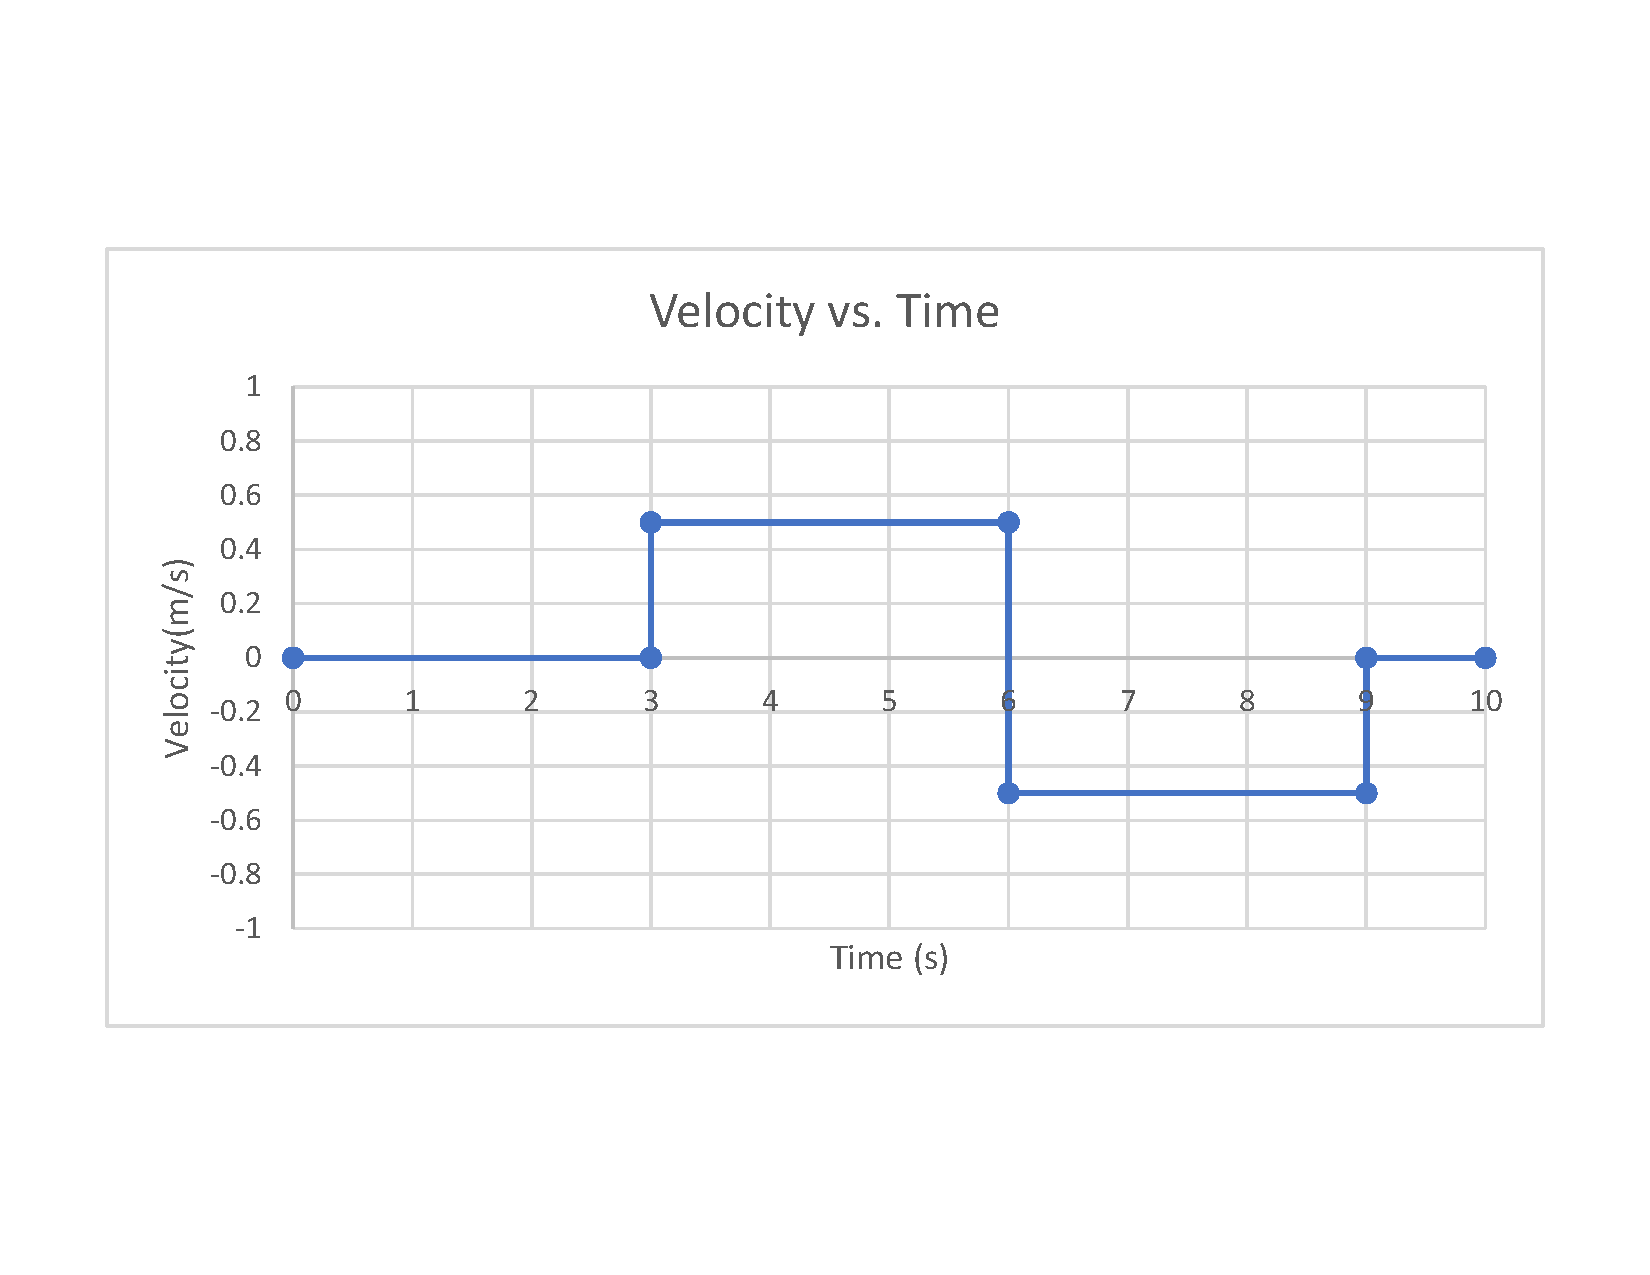
\includegraphics[width=5in]{VelocityvsTimeGraphUsedtoPredict.pdf}\\
\vspace{-10mm}
\textit{Figure 8: The Velocity vs. Time graph used to predict its correlated Position vs. Time graph(Figure 9).}\\
Figure 9\\
\vspace{-10mm}
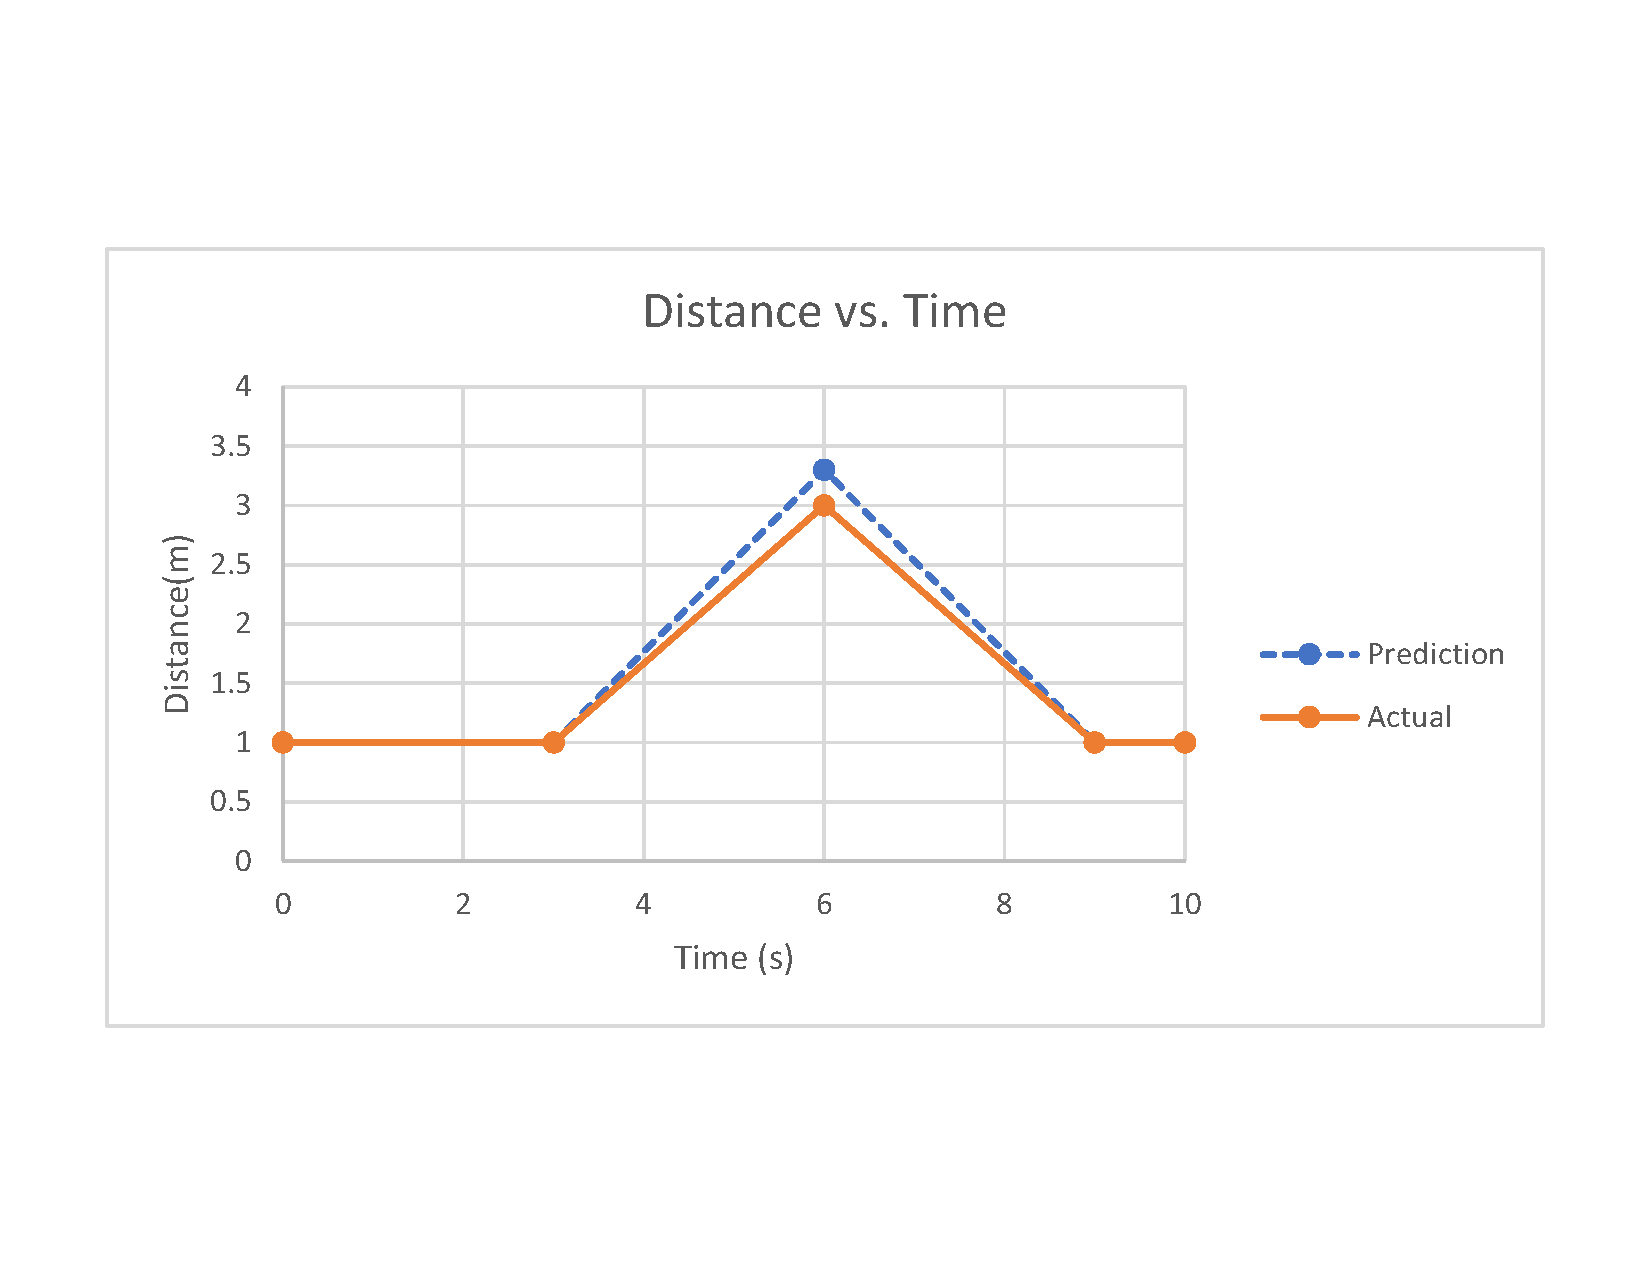
\includegraphics[width=5in]{PositionvsTimeGraphForTheVPrediction.pdf}\\
\vspace{-10mm}
\textit{Figure 9: The predicted and actual Distance vs. Time graph from the Velocity vs. Time graph(Figure 8).}
\newpage
\end{center}

\subsection{Velocity and Acceleration Graphs}

In this section, the acceleration vs. time graph will be introduced and compared to the constant velocity graphs that we have been analyzing through this experiment. Since velocity was the rate at which position changed, it can be predicted that acceleration is the rate at which velocity changes. The mathematical representation would look like this: $a = \frac{dv}{dt}$. Acceleration can also be represented as the second derivative of position in respect to time, the mathematical representation would look like so: $a = \frac{d^2x}{dt^2}$. This section deals with a cart on a "frictionless" ramp to simulate constant velocity.  

\begin{center}
\subsubsection{Diagram of the experiment using a cart}
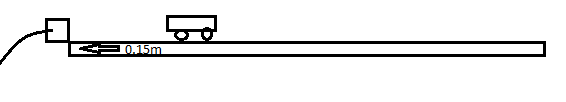
\includegraphics[width=5in]{DIACART.png}\\
\end{center}

With an initial push, the cart stabilized to a constant velocity and produced a distance vs. time graph that was linear and positive sloping and a velocity vs. time graph that had a horizontal line until the moment it hit the end of the ramp. Since the velocity vs. time graph had a constant value through until the point the cart hit the end of the ramp, it was predicted that the acceleration would be 0$\frac{m}{s^2}$. It was predicted because the derivative of any constant value would be zero. When tested the acceleration vs. time graph on the Logger Pro program was indeed a horizontal line at the x-axis, indicating zero acceleration. 

The velocity vectors representing the cart's movement would be pointing in the positive direction because the movement is away from the origin and with the exact same magnitude throughout the cart's motion since the velocity is constant. Acceleration is also a vector quantity, so it can also be represented as a vector. The vector that represents the change in velocity through this system was a zero vector. From the vector the value for acceleration would be 0 $\frac{m}{s^2}$. The acceleration vs. time graph presented by the Logger Pro program and the zero vector of acceleration agree because they both showed acceleration as zero.

\section{Discussion} 

For the majority of this experiment, we were looking at systems with constant velocity and zero acceleration. Analyzing these graphs presented the basis of understanding the effects of change on a distance vs. time graph, velocity vs. time graph, and acceleration vs. time graph in respect to the origin. When given a graph instead of a function, the techniques used in this experiment will help understand the behavior of the motion. The techniques used to analyze and predict graphs will also be applicable in system with variable velocity. 



\section{References}

\hspace{-6.5mm}
Introduction to Motion I Physics 06 Lab\\
Dr. Melanie Lutz



\end{document}
